%
% LaTeX report template 
%

% This is a comment: in LaTeX everything that in a line comes
% after a "%" symbol is treated as comment

\documentclass[11pt, a4paper]{article}
\usepackage{graphicx}
\usepackage{amsmath}
\usepackage{listings}
\usepackage{mathtools}


\title{Assignment7} % Title

\author{Harshavardhan Mudadla\\EE20B084} % Author name

\date{\today} % Date for the report
\begin{document}		
		
\maketitle % Insert the title, author and date
\section{Introduction}
%Create new section;it is autonumbered
This week’s assignment involves the analysis of filters using laplace transforms. Python’s symbolic solving library, sympy is a tool we use in the process to handle our requirements in solving Modified Nodal Analysis equations. Besides this the library also includes useful classes to handle the simulation and response to inputs. Coupled with scipy’s signal module, we are able to analyse both High pass and low pass filters, both second order, realised using a single op amp
\section{Low Pass Filter}
\subsection{Step Response}
\begin{figure}[!tbh]
   	\centering
   	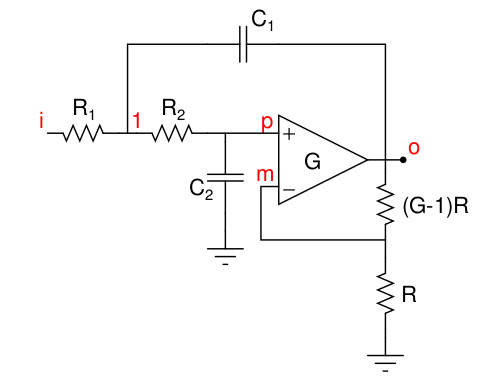
\includegraphics[scale=0.5]{fig6.png}  % Mention the image name within the curly braces. Image should be in the same folder as the tex file. 
   	\caption{A Low-pass filter using an opamp of gain G}
   	\label{fig:sample}
   \end{figure} 
   The low pass filter we use gives the following matrix after simplification of Modified Nodal Equations.
% display math mode
\[
\begin{bmatrix}
    0   & 0 & 1  & -1/G \\
    \frac{-1}{sR_2C_2}  & 1 & 0 & 0\\
    0  & -G & G & 1 \\
    \frac{-1}{R_1} - \frac{1}{R_2} - s*C_1 & \frac{1}{R_2} & 0 & sC_1
\end{bmatrix}
\begin{bmatrix}
    V_1\\
    V_p\\
    V_m \\
    V_o
\end{bmatrix}
=
\begin{bmatrix}
    0 \\
    0 \\
    0 \\
    \frac{-V_i(s)}{R_1} \\
    
\end{bmatrix}
\]
\begin{verbatim}	
s=symbols('s') 
def lowpass(R1,R2,C1,C2,G,Vi): 
  A=Matrix([[0,0,1,-1/G],[-1/(1+s*R2*C2),1,0,0],\
  [0,-G,G,1],[-1/R1-1/R2-s*C1,1/R2,0,s*C1]])
  b=Matrix([0,0,0,-Vi/R1])
  V=A.inv()*b
  return (A,b,V)
\end{verbatim}
Using the lowpass function, we can obtain the impulse response in s-domain for the given values of components as follows :

\begin{verbatim}
A,b,V=lowpass(10000,10000,1e-9,1e-9,1.586,1)
Vo = V[3]
\end{verbatim}

After obtaining the response in its symbolic representation, the following
function is used to convert it into the polynomial representation compatible
with the Signals toolbox of scipy
The following step response is obtained.

\begin{verbatim}	
num,den = fraction(Vo)
c_num = []
c_den = []
isfloat = False
try:
  num=poly(num,s).all_coeffs()
except GeneratorsNeeded:
  c_num = num
  isfloat = True
den=poly(den,s).all_coeffs()
if (isfloat):
  c_den = den
else:
  for i in num:
    c_num.append(float(i))
  c_num = np.array(c_num)

  for i in den:
    c_den.append(float(i))
  c_den = np.array(c_den)
\end{verbatim}

\begin{figure}[!tbh]
   	\centering
   	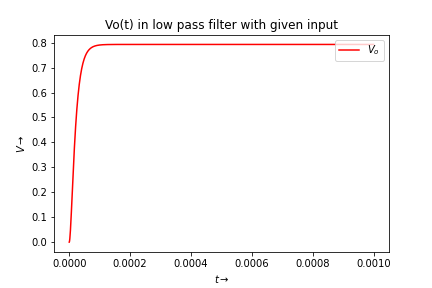
\includegraphics[scale=0.6]{step_respl.png}  % Mention the image name within the curly braces. Image should be in the same folder as the tex file. 
   	\caption{Step response of the lowpass filter}
   	\label{fig:sample}
   \end{figure}

\subsection{Response for a mixed frequency input}
The input is,
$Vi = (sin(2000 \pi t) + cos(2*10^6 \pi t))*u(t)
$
\\
Since the cutoff frequency 1/2$\pi$ MHz, the system is expected to allow the low frequency sine component while attenuating the high frequency cosine component.
\begin{figure}[!tbh]
   	\centering
   	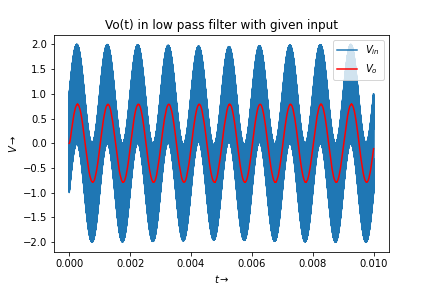
\includegraphics[scale=0.65]{mixed_f_respl.png}  % Mention the image name within the curly braces. Image should be in the same folder as the tex file. 
   	\caption{Output response to a mixed frequency input}
   	\label{fig:sample}
   \end{figure}
\section{High Pass Filter}
\begin{figure}[!tbh]
   	\centering
   	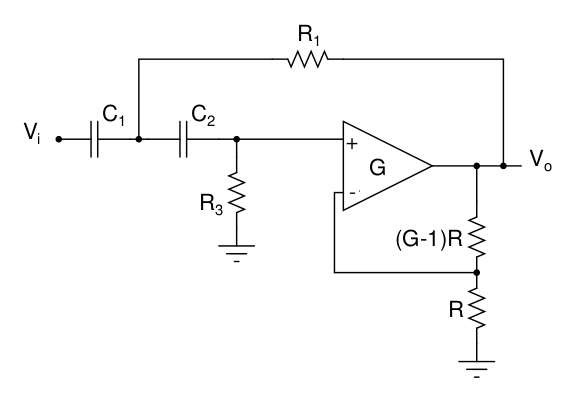
\includegraphics[scale=0.5]{fig7.png}  % Mention the image name within the curly braces. Image should be in the same folder as the tex file. 
   	\caption{A high-pass filter using an op-amp of gain G}
   	\label{fig:sample}
   \end{figure}
   
The high pass filter we use gives the following matrix after simplification of Modified Nodal Equations.
\newline
% display math mode
\[
\begin{bmatrix}
    0   & -1 & 0  & 1/G \\
    \frac{s*C_2*R_3}{1+s*C_2*R_3}  & 0 & -1 & 0\\
    0  & G & -G & 1 \\
    -s*C_2 - \frac{1}{R_1} - s*C_1 & 0 & s*C_2 & \frac{1}{R_1}
\end{bmatrix}
\begin{bmatrix}
    V_1\\
    V_p\\
    V_m \\
    V_o
\end{bmatrix}
=
\begin{bmatrix}
    0 \\
    0 \\
    0 \\
    -V_i(s)*s*C_1 \\
    
\end{bmatrix}\]
\begin{verbatim}
def highpass(R1,R2,C1,C2,G,Vi):
  s=symbols('s')
  A=Matrix([[0,0,1,-1/G],[-1/(1+1/(s*R2*C2)),1,0,0],\
  [0,-G,G,1],[-s*C1-s*C2-1/R1,s*C2,0,1/R1]])
  b=Matrix([0,0,0,-Vi*s*C1])
  V=A.inv()*b
  return (A,b,V)
\end{verbatim}
The magnitude response, as expected, is that of a high pass filter, with
cut-off frequency at 1/2$\pi$ MHz is given below.
\begin{figure}[!tbh]
   	\centering
   	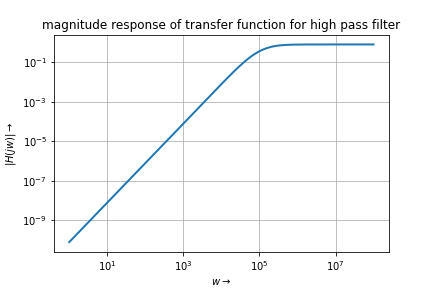
\includegraphics[scale=0.7]{mag_response.png}  % Mention the image name within the curly braces. Image should be in the same folder as the tex file. 
   	\caption{$|H(jw)|$ vs w in loglog scale}
   	\label{fig:sample}
   \end{figure}
   \subsection{Response to damped sinusoid}
   Consider the following damped sinusoids, $v_in = e^{-0.5t}sin(2 \pi 10^3t)$ and $v_in = e^{-0.5t}sin(2 \pi 10^8t)$.
   \newline
   The high pass filter is expected to attenuate the low frequency sinusoid.
The system should allow frequencies such as $10^8$ Hz as they are above the
cut-off frequency.
\begin{figure}[!tbh]
   	\centering
   	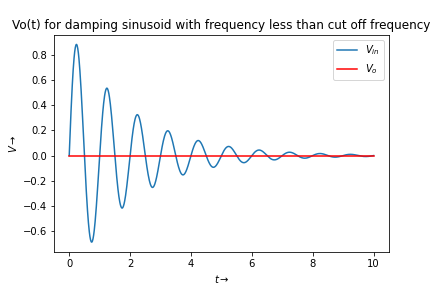
\includegraphics[scale=0.7]{damp_l.png}  % Mention the image name within the curly braces. Image should be in the same folder as the tex file. 
   	\caption{High-pass filter response for $10^3$ Hz sinusoid input}
   	\label{fig:sample}
   \end{figure}
  \begin{figure}[!tbh]
   	\centering
   	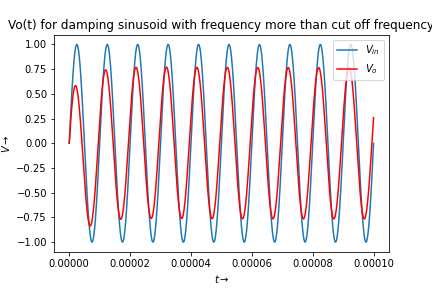
\includegraphics[scale=0.7]{damp_h.png}  % Mention the image name within the curly braces. Image should be in the same folder as the tex file. 
   	\caption{High-pass filter response for $10^8$ Hz sinusoid input}
   	\label{fig:sample}
   \end{figure}
   \newpage
   \subsection{Step Response}
   \begin{figure}[!tbh]
   	\centering
   	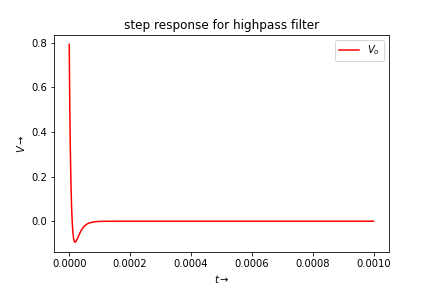
\includegraphics[scale=0.65]{step_resph.png}  % Mention the image name within the curly braces. Image should be in the same folder as the tex file. 
   	\caption{Step response of high pass filter}
   	\label{fig:sample}
   \end{figure}
   \newpage
 \section{Conclusion}
 For a mixed frequency sinusoid as
input, it was found that the filter suppressed the high frequencies while
allowing the low frequency components. Similarly, a high pass filter was
implemented using an op-amp with the same gain. The magnitude response
of the filter was plotted and its output was analysed for damped sinusoids.
\end{document}
